After unblinding the full data, the resulting vertex distribution is shown in Figure~\ref{fig:zVm_ub}.

\begin{figure}[htb]
  \centering
      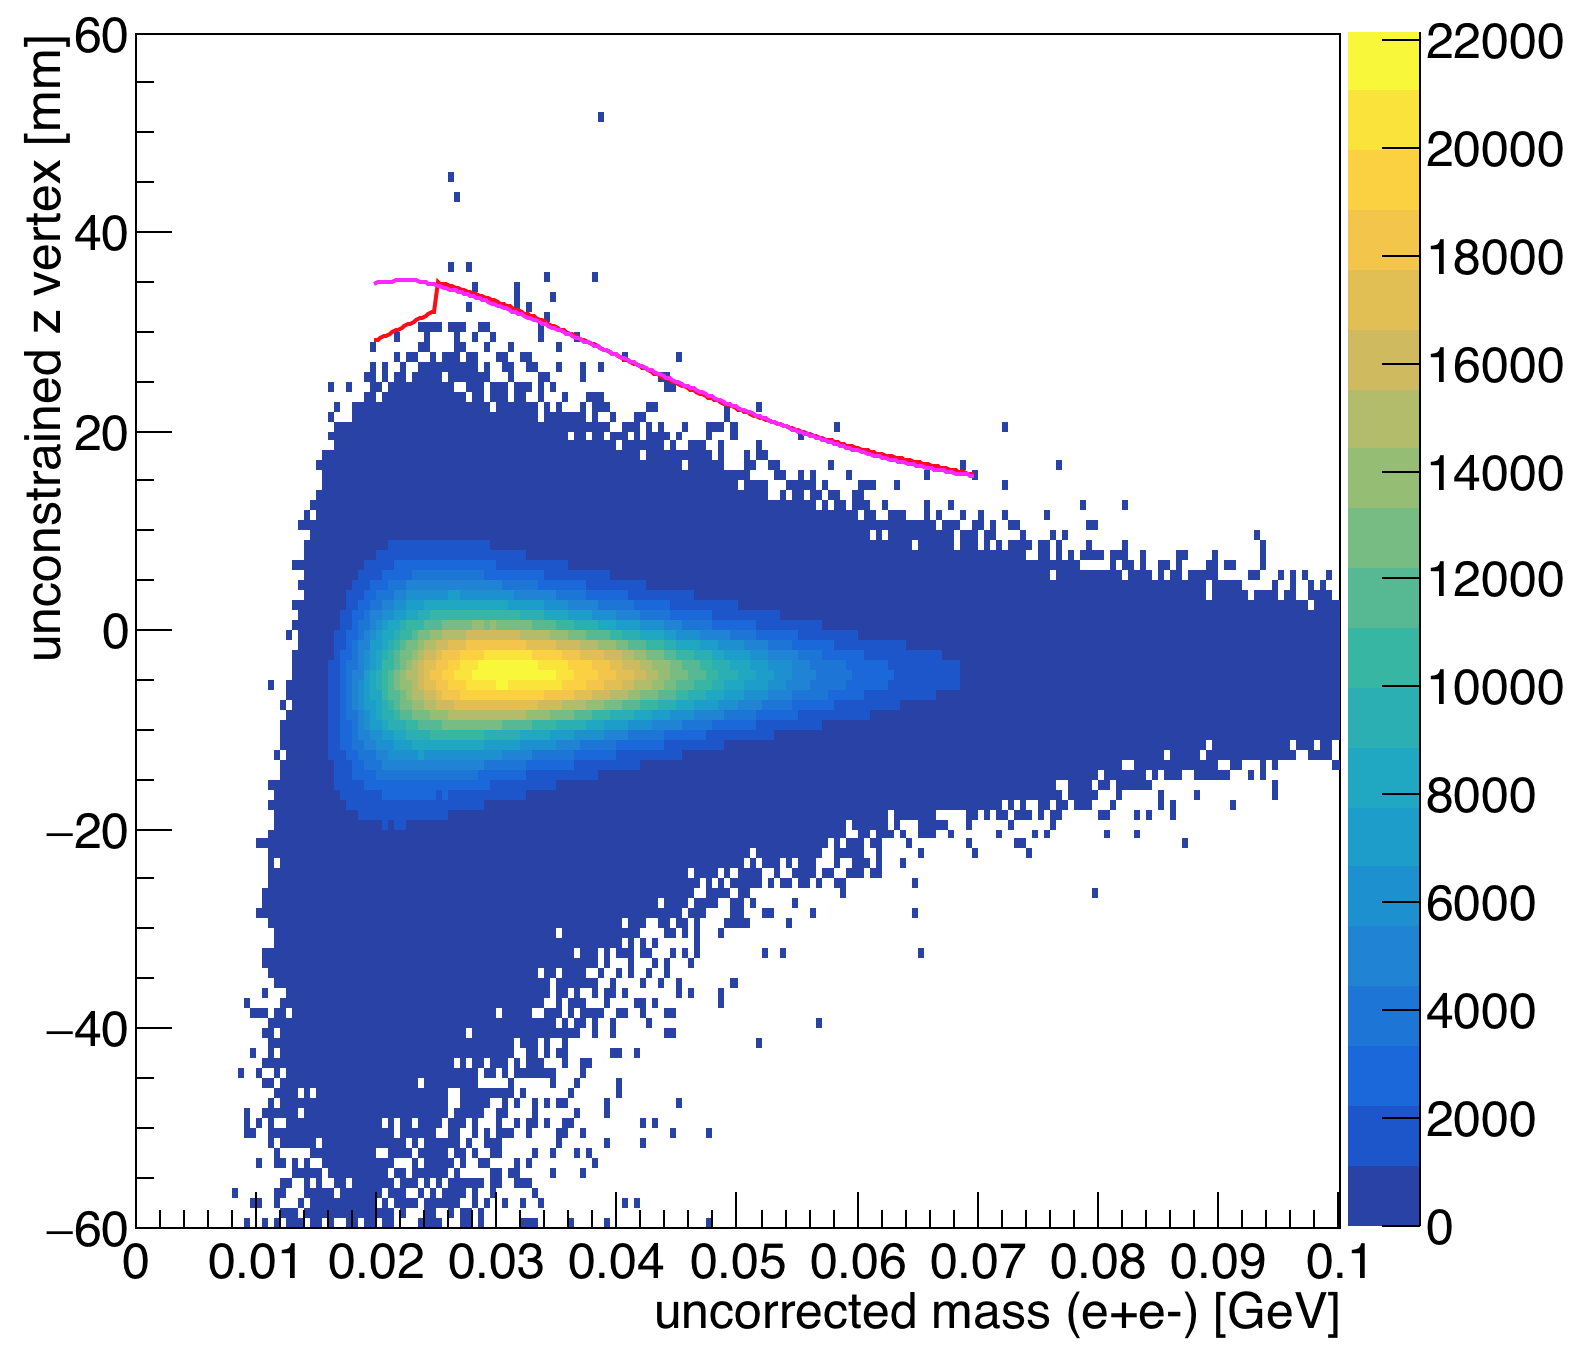
\includegraphics[width=0.75\textwidth]{pics/results/zVm_ub_L1L1.png}
  \caption[Vertex position vs mass for the 100$\%$ L1L1 data at 0.5~mm]{The unconstrained $z$ vertex position is shown as a function of the corrected mass of the $e^+e^-$ pair. The $zCut$ as measured for this data is shown in red and corresponds to where there is less than 0.5 background event beyond. The projected $zCut$ from the 10$\%$ of the data is shown in magenta. The relevant mass range used to fit $zCut$ is from 0.02-0.08~GeV based on measured statistics.}
  \label{fig:zVm_ub}
\end{figure} 

The projected $zCut$ from the 10$\%$ sample agrees reasonably well with the $zCut$ measured from the full data vertex distribution. The $zCut$ is supposed to correspond to where one would measure less than 0.5 background events in the resolution-sized mass bin. As one can see from Figure~\ref{fig:zVm_ub}, there are significantly more events in the high $z$ region. The distribution of these events as a function of mass is shown in Figure~\ref{fig:highz_mass}.

\begin{figure}[htb]
  \centering
      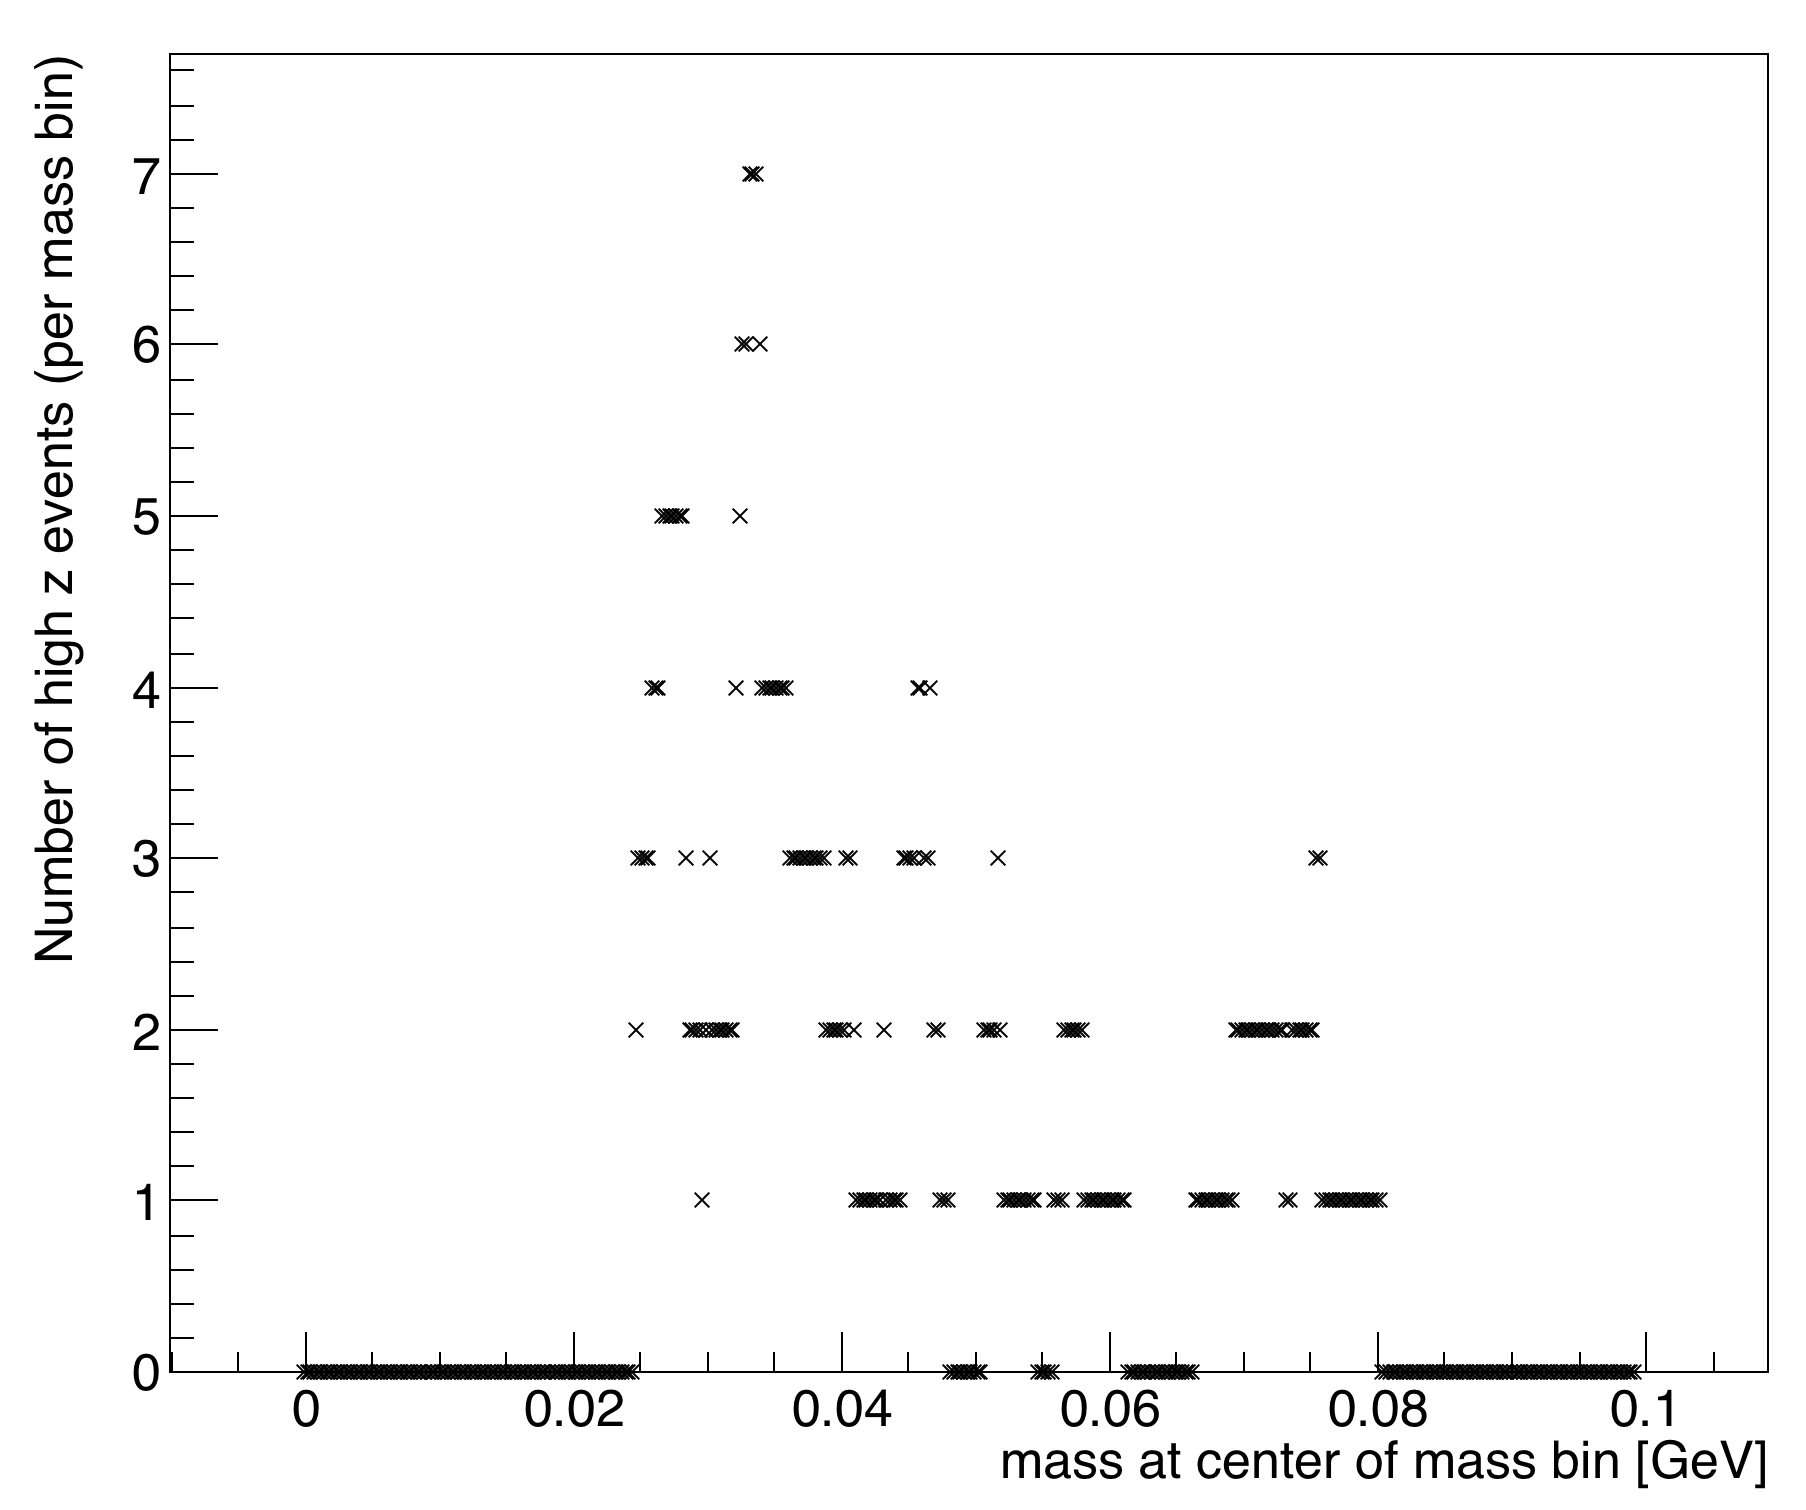
\includegraphics[width=0.75\textwidth]{pics/results/highz_v_mass.png}
  \caption[High $z$ events as a function of mass]{The high $z$ events from the full data set are shown as a function of their mass. Many of the events are plotted several times for the number of mass-resolution sized mass bins that they appear in. The highest number appear around 34~MeV, but the background is generally much higher than predicted across the full, measurable mass range.}
  \label{fig:highz_mass}
\end{figure} 

From choosing $zCut$ to correspond to 0.5 background events per mass bin, one would expect 6 high $z$ events across the range from 0.02 to 0.08~GeV. In reality, there are 24 events across this range. The distribution in mass peaks for the mass bin centered at 34~MeV, but is generally much higher than predicted across the full, measurable range. \\
\indent Because this is the full data that we are looking at, and there could potentially be a heavy photon in the data set, we must be extremely careful in how we choose to characterize the excess background events. If we assume that the heavy photon will only appear in one mass bin, then one can very roughly estimate the measured background for a particular mass hypothesis by excluding events that fall in its mass range and measuring the average number of background events elsewhere. The average number of background events per mass bin, excluding those events in the mass hypothesis, is shown in Figure~\ref{fig:highz_newbg}.
 
\begin{figure}[htb]
  \centering
      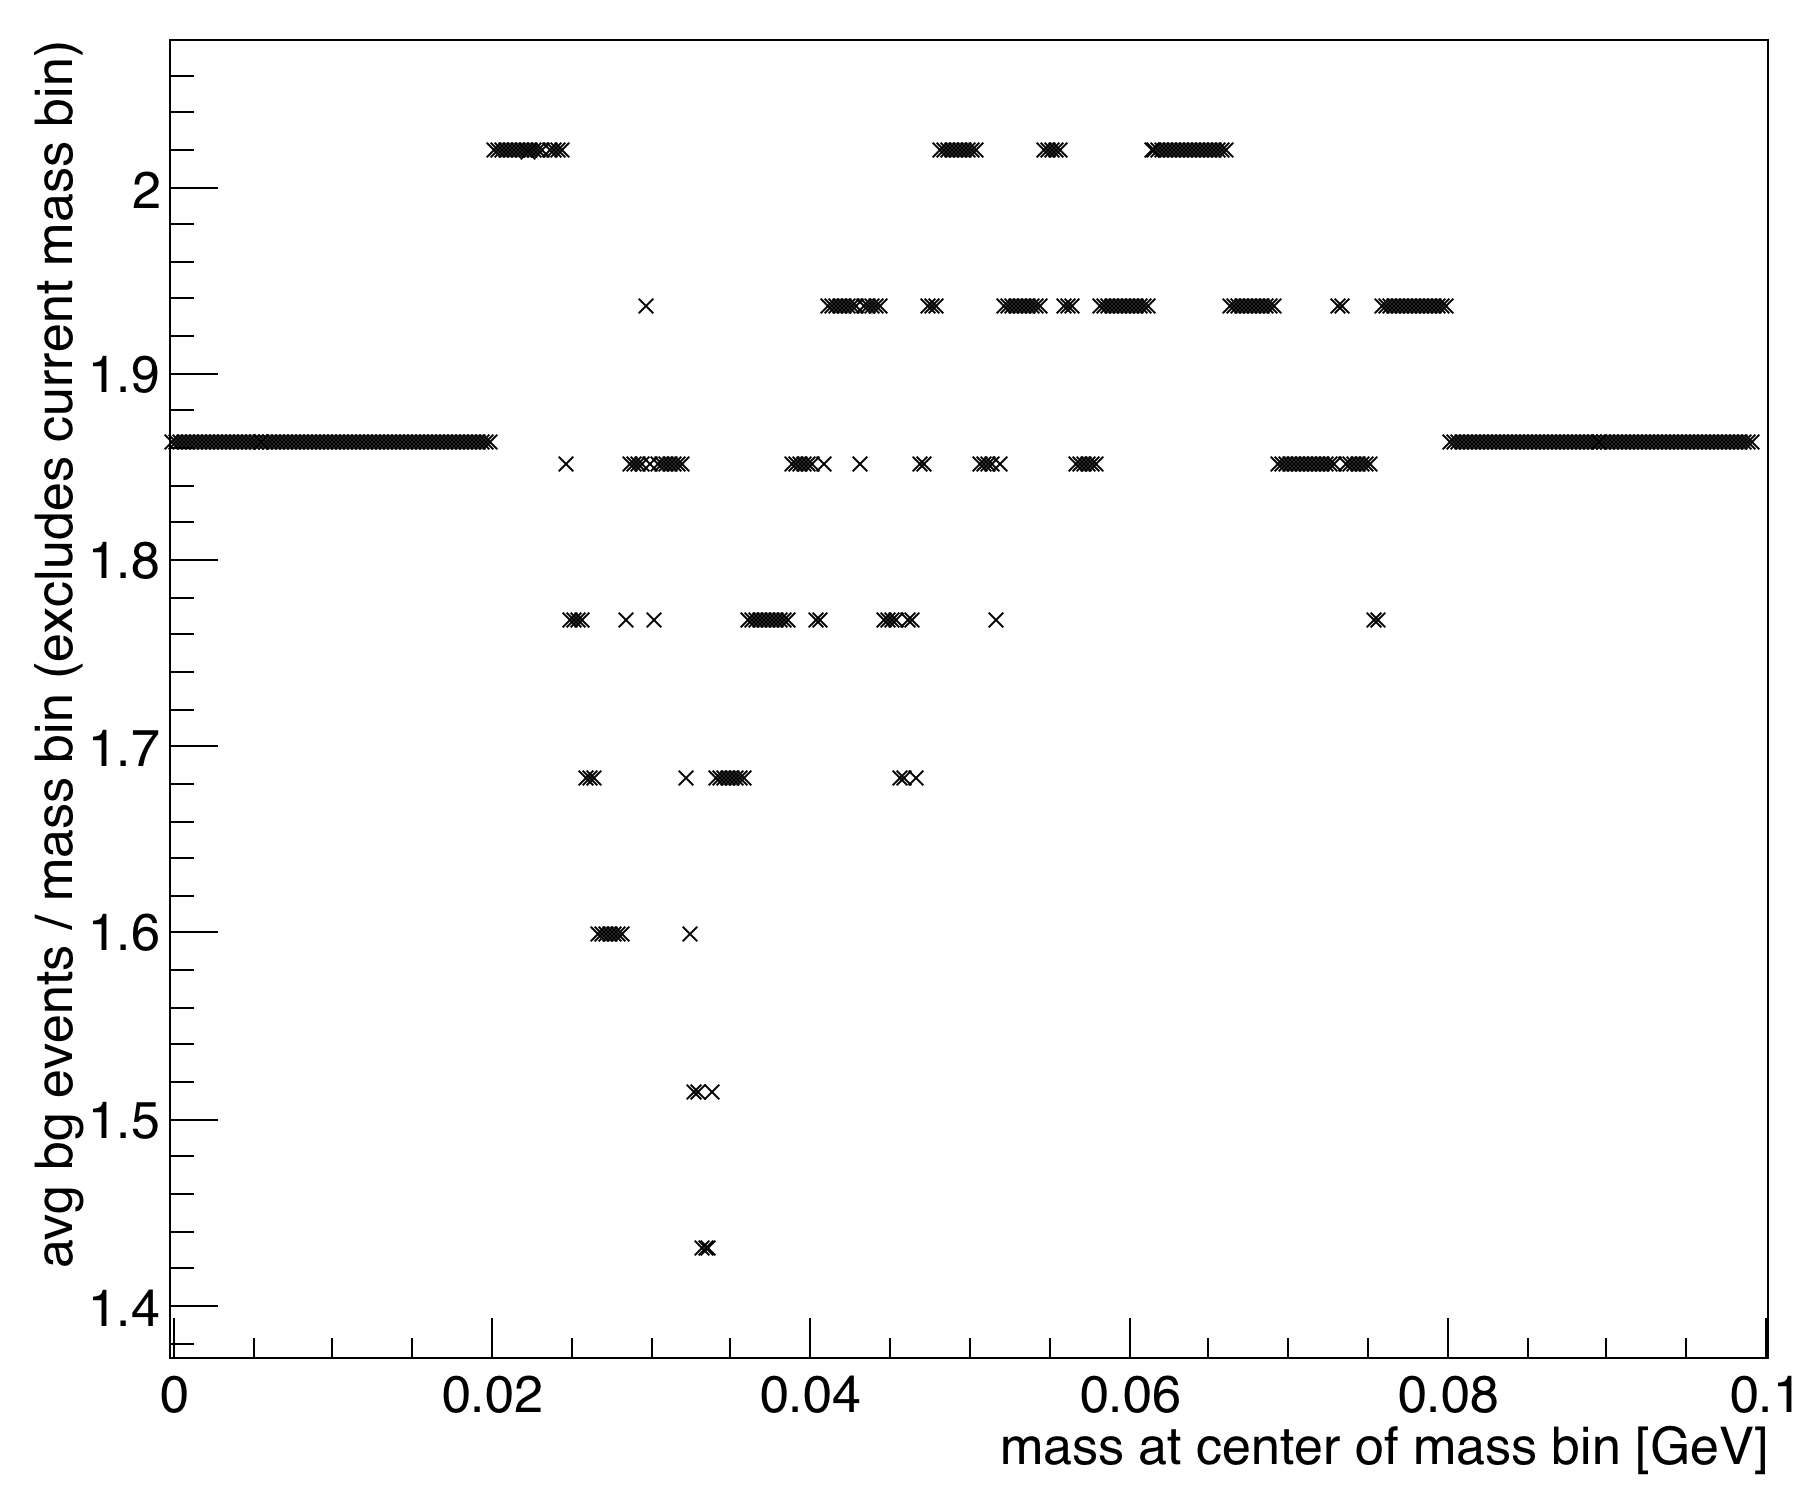
\includegraphics[width=0.75\textwidth]{pics/results/highz_avgBG.png}
  \caption[Re-characterization of the excess background]{The background events per mass bin are shown for each mass hypothesis by excluding the events that fall in that mass resolution-limited bin. This assumes that the heavy photon will fall in any one bin and results in a conservative background estimate for each bin.}
  \label{fig:highz_newbg}
\end{figure} 

The re-characterized background average ranged between 1.4 just over 2 background events per mass bin. This is significantly higher than the proposed 0.5 background events per mass bin. Ultimately, this distribution should be simulated and re-fit to be included in the $zCut$ calculation. For now, this is a sufficiently conservative estimate of the excess background and can be used to obtain the p-value associated with each mass hypothesis. \\
\indent The p-value is the probability in a background-only scenario to measure an apparent signal as significant as the data. Using the background as estimated from Figure~\ref{fig:highz_newbg}, we measure the following p-values in the fluctuations as shown in Figure~\ref{fig:highz_pval}.

\begin{figure}[htb]
  \centering
      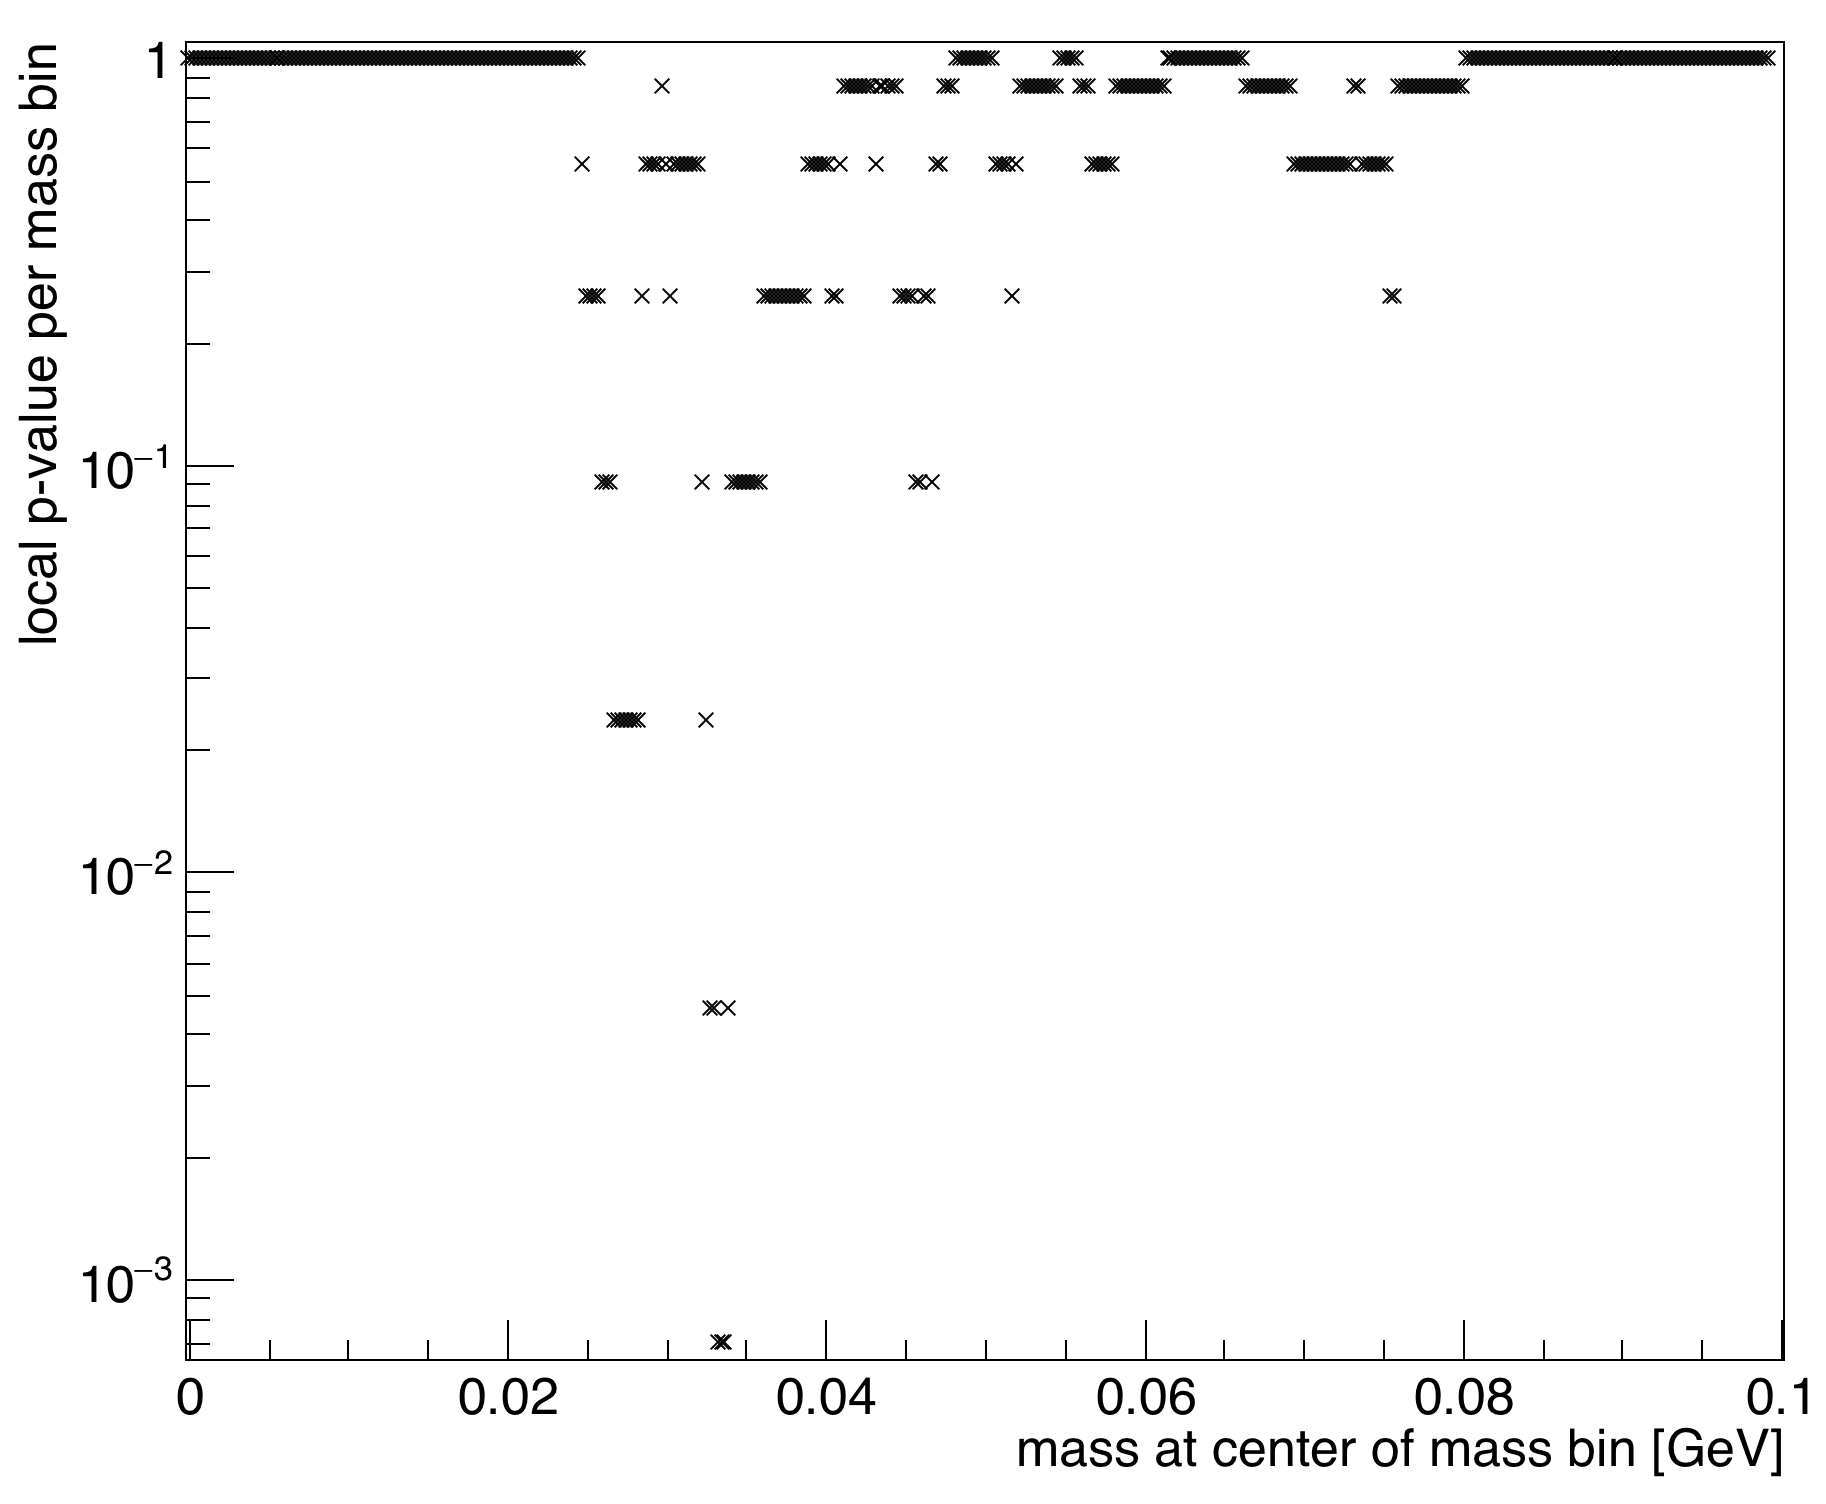
\includegraphics[width=0.75\textwidth]{pics/results/highz_pval.png}
  \caption[Local p-values for the L1L1 dataset]{The local p-values for each mass hypothesis using the data-characterized background estimate is shown. The p-value shows how well each hypothesis agrees with the background only model. The most significant p-value has a value of 0.00071 at approximately 34~MeV as this bin contains 7 high $z$ background events.}
  \label{fig:highz_pval}
\end{figure} 

The p-values shown in Figure~\ref{fig:highz_pval} are considered t be "local" p-values as they only consider the significance of the events in a specific mass hypothesis and do not look at the significance of those events across the range of the full data. This is known as the Look Elsewhere Effect. In order to account for this effect, the local p-values need to be mapped to global p-values in order to properly ascertain the significance of any of these fluctuations. The global p-value will always yield something smaller than the local p-value by definition. By generating 10,000 toy vertex distributions and finding the most significant p-value in each simulation, one can obtain the mapping from local to global p-values. The mapping using toy distributions of the L1L1 0.5~mm data is shown in Figure~\ref{fig:pval_map}.

\begin{figure}[htb]
  \centering
      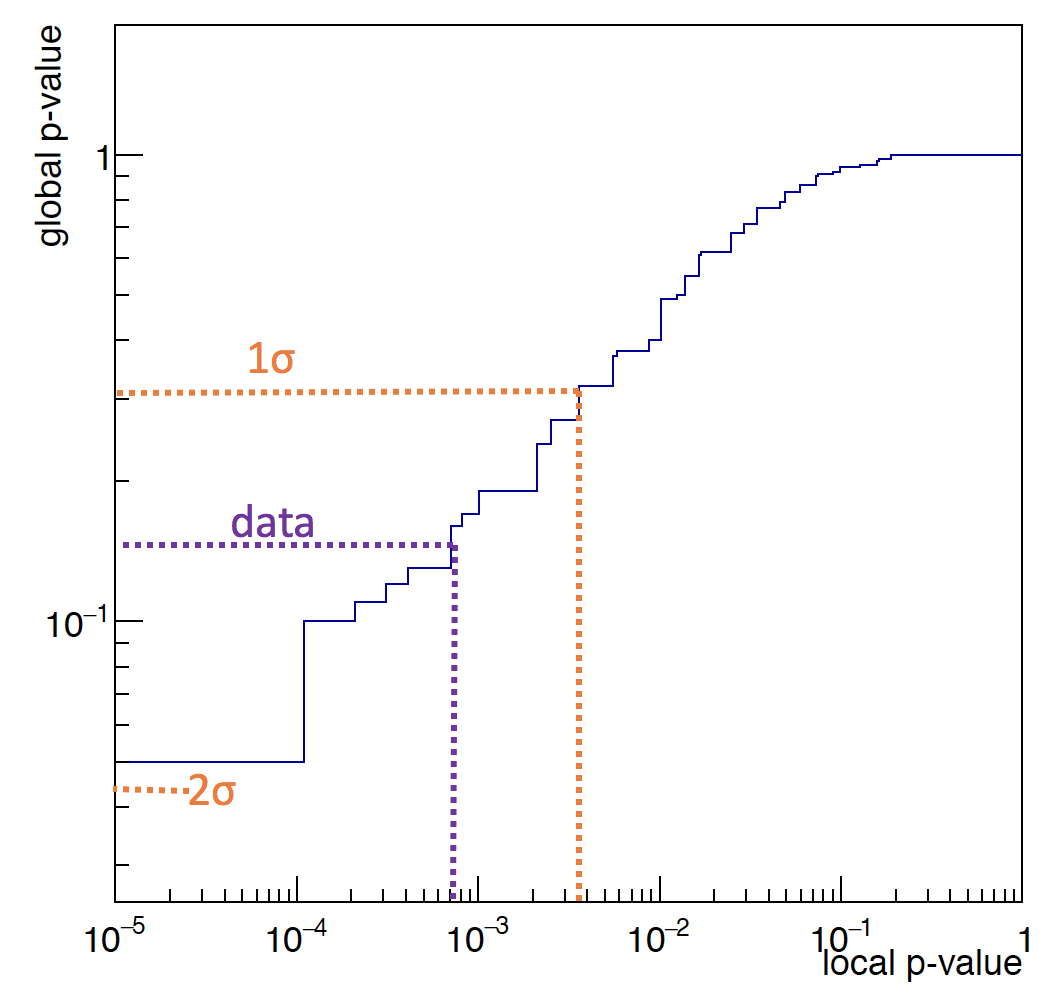
\includegraphics[width=0.75\textwidth]{pics/results/pvalMap.png}
  \caption[Mapping of local to global p-values]{The local to global p-value mapping is shown using 10,000 toy distributions modeled from the data. The orange dashed lines indicate the approximate locations of the global p-values as a significance in terms of a Gaussian fluctuation. The purple dashed line indicates the global p-value of the most significant fluctuation from the data (with local p-value of 0.00071) is 0.13. This translates to a Gaussian significance of 1.12$\sigma$.}
  \label{fig:pval_map}
\end{figure} 

In Figure~\ref{fig:pval_map}, the global p-values account for the significance of the fluctuations over the range of the data set. The most significant local p-value corresponds to a global p-value of 0.13 which can be expressed as a Gaussian significance of 1.12$\sigma$. Therefore, in accounting for the presence of the unanticipated excess background, we did not observe any signal significance. \\
\indent Additionally, we can see how significantly the measured excess background vertices are with respect to the background model by transforming the fit into a cumulative distribution function. We can see the deviation of the measured $z$ vertex as the quantile of $1-e^{(z_{cut}-z)/l}$. For high $z$ events that agree well with the background hypothesis, the quantile is closer to 0. Those events that deviate with respect to the background hypothesis will be closer to 1. These values are shown in Figure~\ref{fig:highz_quantile}.

\begin{figure}[htb]
  \centering
      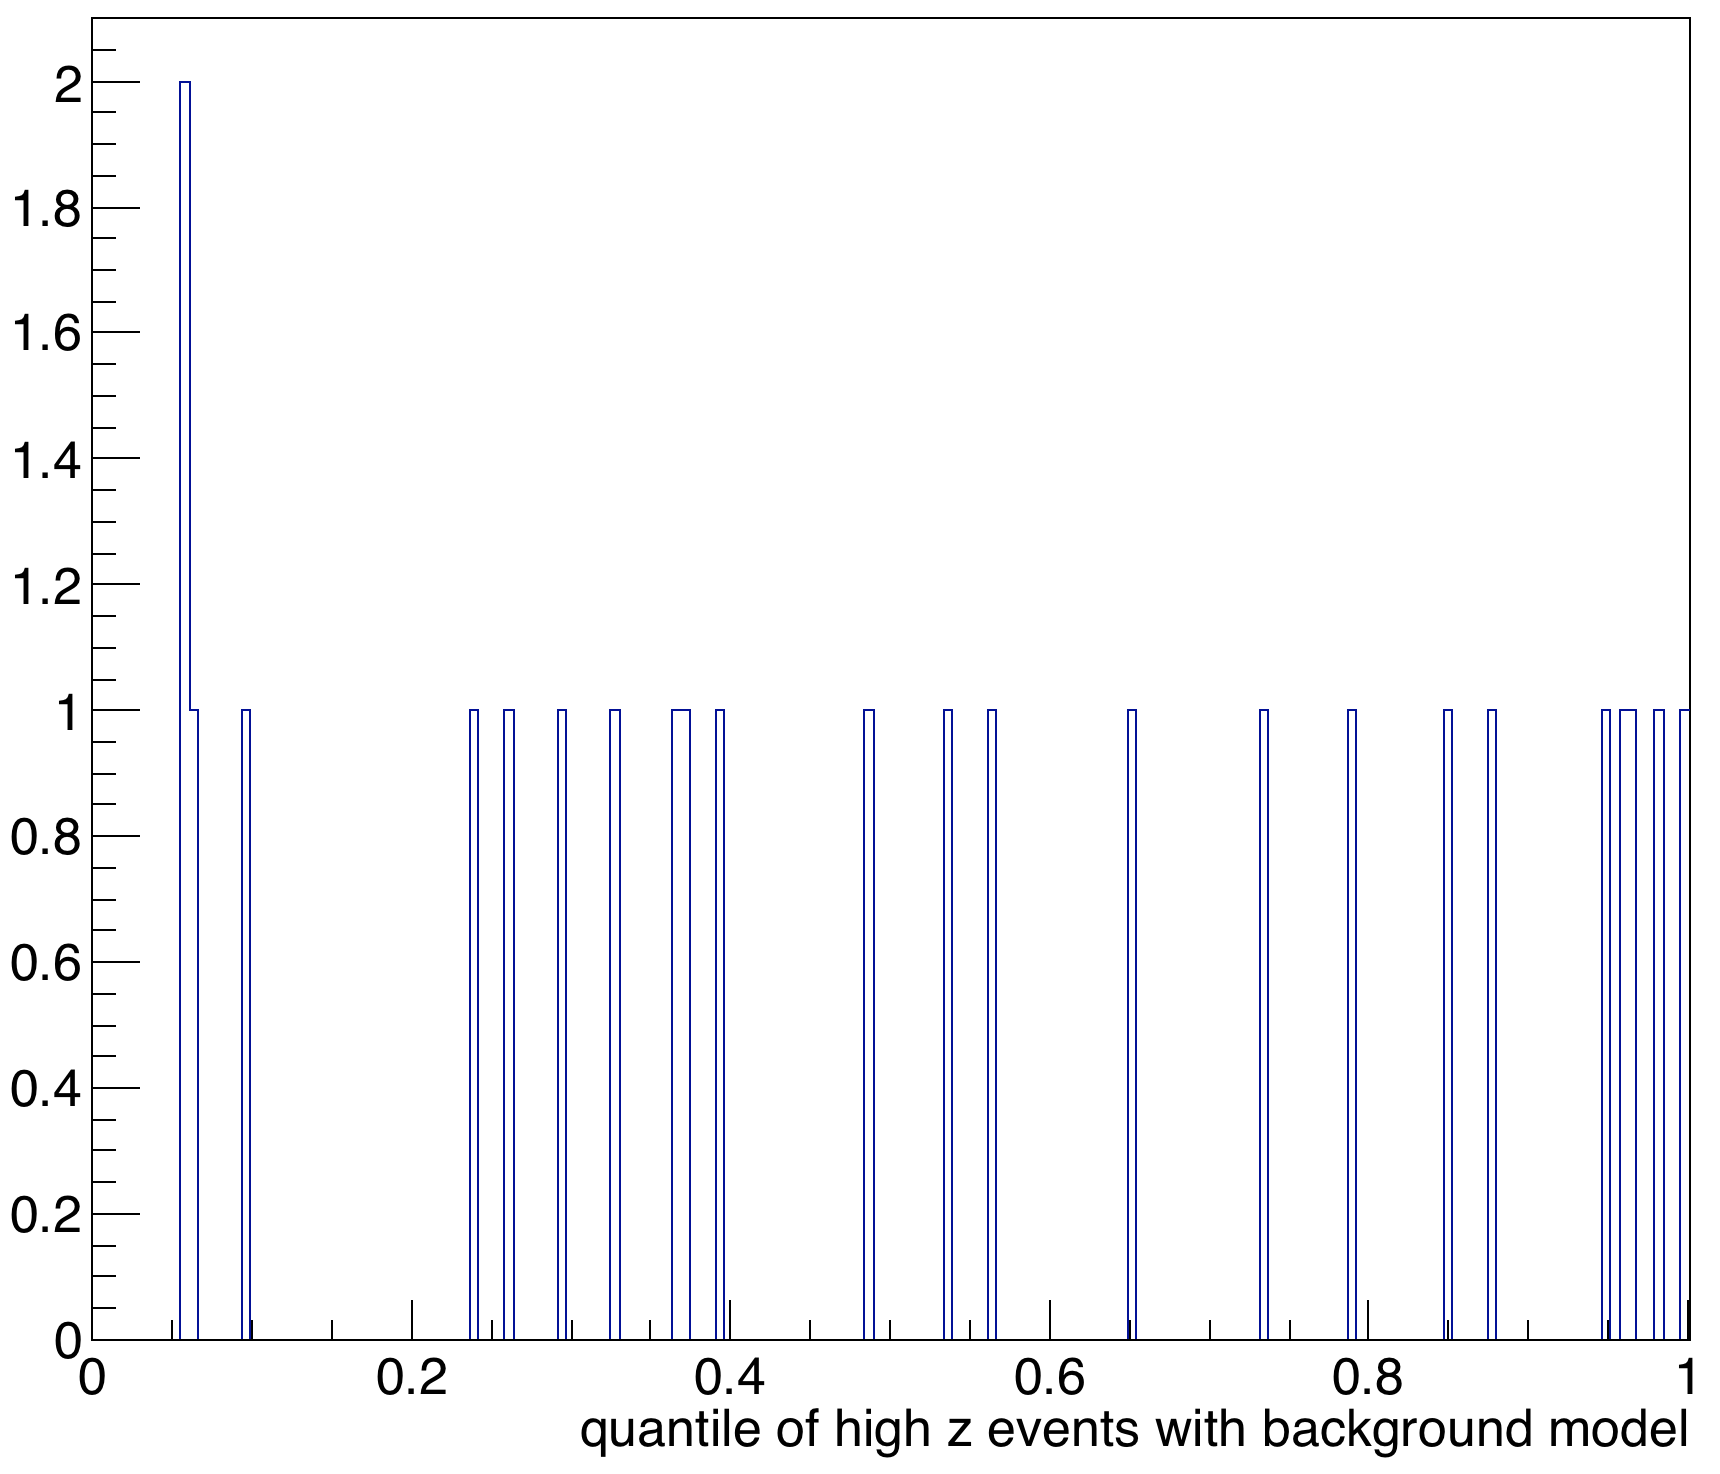
\includegraphics[width=0.75\textwidth]{pics/results/highz_quantiles.png}
  \caption[Deviation of the measured high $z$ event from the background $zCut$]{The deviation of the measured high $z$ event from the background is defined by the quantile of the cumulative distribution function $1-e^{(z_{cut}-z)/l}$. Events that are consistent with the hypothesis are close to 0 while those events that differ greatly from the hypothesis are closer to 1.}
  \label{fig:highz_quantile}
\end{figure} 

There are five events that are clustered close to 1 having a significant deviation with respect to the background $zCut$ hypothesis. These remainder of the events are spread fairly evenly across all mass hypotheses. These events with the greatest difference will lie farthest from the $zCut$ and are mostly centered around the 34~MeV mass bin which also contains the largest signal fluctuation. In order to obtain the correct amount of high $z$ events across the distribution, one would need to move the $zCut$ downstream by 4~mm. This still have one mass bin containing 3~events. By moving the $zCut$ 5~mm downstream, no mass resolution-sized bin would contain more than 2~events. 

\subsection{Discussion of the L1L1 data with the SVT at $\pm$1.5~mm}
The 1.5~mm L1L1 data set is much lower in statistics than the 0.5~mm data but also has significantly less background events. The full vertex distribution is shown in Figure~\ref{fig:zVm1p5_ub}.

\begin{figure}[htb]
  \centering
      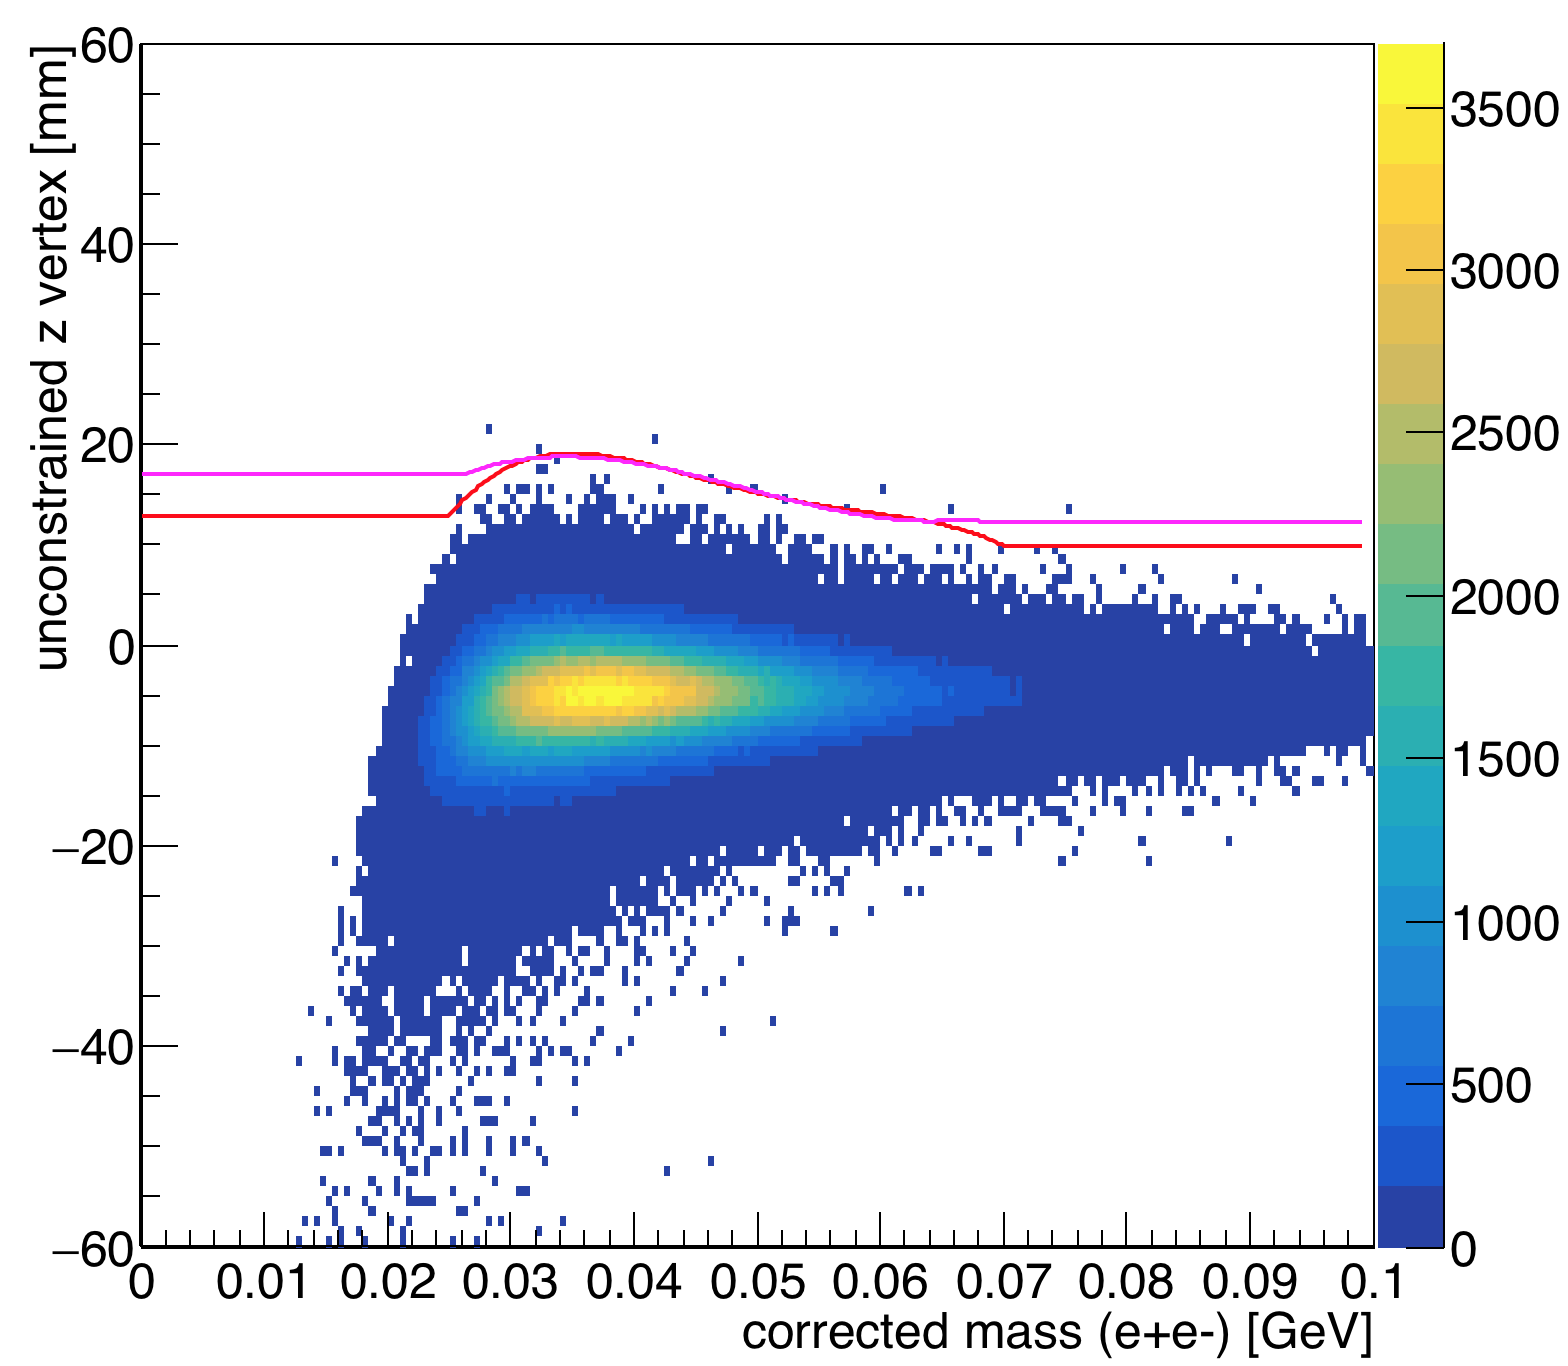
\includegraphics[width=0.75\textwidth]{pics/results/zVm_1p5mm.png}
  \caption[Vertex position vs mass for the 100$\%$ L1L1 data at 1.5~mm]{The unconstrained $z$ vertex position is shown as a function of the corrected mass of the $e^+e^-$ pair in events with SVT at $\pm1.5$~mm from the beam. The $zCut$ as measured for this data is shown in red and corresponds to where there is less than 0.5 background event beyond. The projected $zCut$ from the 10$\%$ of the data is shown in magenta. The relevant mass range used to fit $zCut$ is from 0.025-0.07~GeV based on measured statistics.}
  \label{fig:zVm1p5_ub}
\end{figure} 

If we consider the high $z$ background in the 1.5~mm data set, we see that the average number of background events throughout the mass range is around 0.8 events per resolution-sized mass bin. Additionally, there are at most 2 events in a single one of the resolution-sized bins. If we exclude the three events that lie on the $zCut$ (either by agreement with the background model or moving the $zCut$ by 1~mm farther downstream), then we obtain an average of 0.51 events per resolution-sized mass bin. This seems to indicate that most of the high $z$ background in the 0.5~mm data is coming from beam scatters in the dead region of Layer 1.  